% v2-acmlarge-sample.tex, dated March 6 2012
% This is a sample file for ACM large trim journals
%
% Compilation using 'acmlarge.cls' - version 1.3, Aptara Inc.
% (c) 2011 Association for Computing Machinery (ACM)
%
% Questions/Suggestions/Feedback should be addressed to => "acmtexsupport@aptaracorp.com".
% Users can also go through the FAQs available on the journal's submission webpage.
%
% Steps to compile: latex, bibtex, latex latex
%
\documentclass[acmtap]{acmlarge}

% Metadata Information
\acmVolume{2}
\acmNumber{3}
\acmArticle{1}
\articleSeq{1}
\acmYear{2010}
\acmMonth{5}

% Package to generate and customize Algorithm as per ACM style
\usepackage[ruled]{algorithm2e}
\usepackage{graphicx}
\usepackage{listings}
\usepackage{amsmath}
\SetAlFnt{\algofont}
\SetAlCapFnt{\algofont}
\SetAlCapNameFnt{\algofont}
\SetAlCapHSkip{0pt}
\IncMargin{-\parindent}
\renewcommand{\algorithmcfname}{ALGORITHM}

% Page heads
\markboth{S. Sammak}{Solving Incompressible Navier-Stokes Equation in Parallel  }

% Title portion
\title{ME2055 Final Project \\(Solving Incompressible Navier-Stokes Equation in Parallel)}
\author{Shervin Sammak \affil{University of Pittsburgh}
}
% NOTE! Affiliations placed here should be for the institution where the
%       BULK of the research was done. If the author has gone to a new
%       institution, before publication, the (above) affiliation should NOT be changed.
%       The authors 'current' address may be given in the "Author's addresses:" block (below).
%       So for example, Mr. Fogarty, the bulk of the research was done at UIUC, and he is
%       currently affiliated with NASA.

\begin{abstract}
This homework provides a overview of numerical solutions to the incompressible Navier-Stocks over a step profile. FTCS and point Gauss-Seidel are developed to solve unsteady vorticity equation and stream function equation respectively. To illustrate the effect of parallelization of the code, OpenMP (Shared Memory) is considered.   
\end{abstract}

\category{}{ME2055- Spring 2014}{}

% At a minimum you need to supply the author names, year and a title.
% IMPORTANT:
% Full first names whenever they are known, surname last, followed by a period.
% In the case of two authors, 'and' is placed between them.
% In the case of three or more authors, the serial comma is used, that is, all author names
% except the last one but including the penultimate author's name are followed by a comma,
% and then 'and' is placed before the final author's name.
% If only first and middle initials are known, then each initial
% is followed by a period and they are separated by a space.
% The remaining information (journal title, volume, article number, date, etc.) is 'auto-generated'.

\begin{document}



\maketitle

% Head 1
\section{Introduction}
An important issue in fluid dynamics is the study of flow separation, which results in a global change of the flow field topology. One example is the flow separation and recirculation caused by a sudden contraction in a channel, in the form of a backward facing step. Incompressible Navier-Stokes equation is used and numerically applied to a 2D domain using uniform Cartesian mesh. 

\begin{figure}[htb]
  \centering
  \begin{tabular}{c}

    % Requires \usepackage{graphicx}

    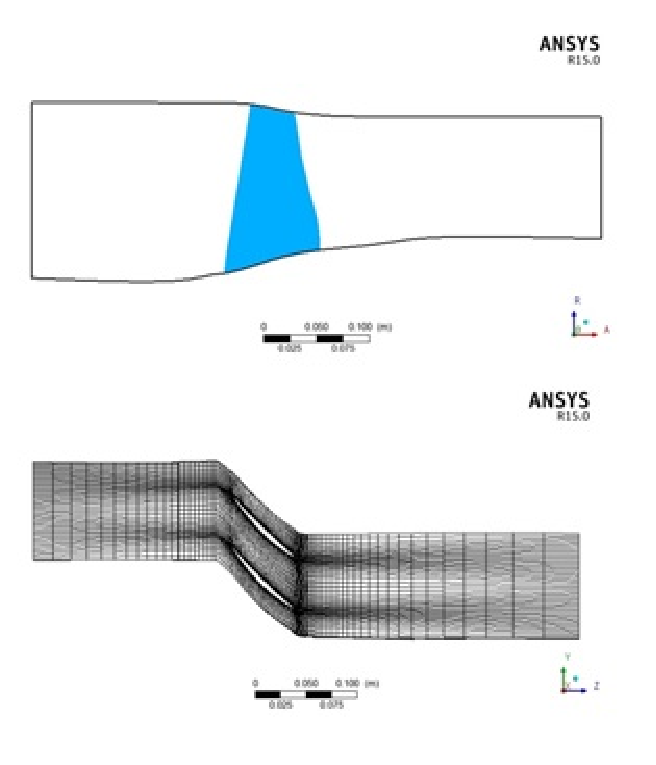
\includegraphics[width=160mm]{13.eps} 


  \end{tabular}
\label{figur}\caption{Schematic of domain and Mesh grids.}
\end{figure}

The governing equation are given by the vonricity equation 
\begin{eqnarray}
\frac{\partial \omega}{\partial t} + u \frac{\partial \omega}{\partial x}+v \frac{\partial \omega}{\partial y} &=&  \frac{1}{Re} ( \frac{\partial^2 \omega}{\partial x^2} + \frac{\partial^2 \omega}{\partial y^2})
\end{eqnarray}

and the stream function equation  

\begin{eqnarray}
\frac{\partial^2 \psi}{\partial x^2} + \frac{\partial^2 \psi }{\partial y^2} &=& -\omega
\end{eqnarray}


\section{Numerical Scheme}
Several numerical schemes for the solution of the vorticity transport equation have been reviewed in [1]. The FTCS scheme is used here to develop a numerical code. The formulation is rearranged as follows

\begin{eqnarray}
\omega_{i,j}^{n+1} &=& \omega_{i,j}^{n} - \frac{\Delta t}{2\Delta x} u_{i,j}^{n} (\omega_{i+1,j}^{n} - \omega_{i-1,j}^{n} ) -  \frac{\Delta t}{2\Delta y} v_{i,j}^{n} (\omega_{i+1,j}^{n} - \omega_{i-1,j}^{n} )  \nonumber \\
 &+& \frac{\Delta t}{(\Delta x)^2} \frac{1}{Re} (\omega_{i+1,j}^{n} -2\omega_{i,j}^{n} \omega_{i-1,j}^{n} ) + \frac{\Delta t}{(\Delta y)^2} \frac{1}{Re} (\omega_{i,j+1}^{n} -2\omega_{i,j}^{n} \omega_{i,j-1}^{n} )
\end{eqnarray}

The stream function equation is an elliptic equation, and any one of the iterative schemes in [1] can be used to botain a solution. The point Gauss-Seidel scheme, given by Eq. (4) is used in numerical code.

\begin{eqnarray}
\psi_{i,j}^{k+1} = \frac{1}{1+ \beta^2} \Big[(\Delta x)^2 \omega_{i,j}^{n+1}+ \psi_{i+1,j}^{k}+ \psi_{i-1,j}^{k+1}+ \beta^2 (\psi_{i,j+1}^{k}+ \omega_{i,j-1}^{k+1})\Big]
\end{eqnarray}

A step by step solution procedure us summarized as follows. \\
1- Initialize all the variables. \\
2- Update the vorticity within the domain by application of Eq. (3). \\
3- Solve Eq. (3) for the vorticity within the domain at the time level n+1. \\
4- Solve Eq. (4) for the stream function at the n+1 time level. Since an iterative scheme is used, a convergence criterion must be set. \\
5- Update the value of stream function where Neumann boundary condition is used. \\
6- Update the values of the vorticity at the boundaries. \\
7- Update the velocity field within the domain using finite difference equation for $u$ and $v$ (Eq. (5-6)). \\
8- Go to step 2 and repeat the computation up to specified final time level. 

\begin{eqnarray}
u_{i,j}^{n+1} &=& \frac{\psi_{i,j+1}^{n+1}- \psi_{i,j-1}^{n+1}}{2 \Delta y} \\
v_{i,j}^{n+1} &=& - \frac{\psi_{i+1,j}^{n+1}- \psi_{i-1,j}^{n+1}}{2 \Delta y} \\
\omega &=& \frac{\partial v}{\partial x} - \frac{\partial u}{\partial y} \nonumber \\
\omega &=& \frac{v_{i+1,j}- v_{i-1,j}}{2 x} - \frac{u_{i+1,j}-u_{i-1,j}}{2y}
\end{eqnarray}



During the computations as a measure of convergence to the steady state, I monitored residual for stream function and vorticity. The residual parameter, $RES_\psi$ and $RES_\omega$ is normalized by the representative value at the previous time step. This then provides an indication of the maximum percent change in $\psi$ in each iteration step.

\begin{eqnarray}
RES_\psi= \sum_{i=2,j=2}^ {i=n-1,j=m-1} \Big | \cfrac{  \psi_{i,j}^{k+1} -  \psi_{i,j}^{k}}{\psi_{i,j}^{k}} \Big | \nonumber \\
RES_\omega= \sum_{i=2,j=2}^ {i=n-1,j=m-1} \Big | \cfrac{  \omega_{i,j}^{k+1} -  \omega_{i,j}^{k}}{\omega_{i,j}^{k}} \Big |
\end{eqnarray}

In my calculations, I considered that convergence was achieved when $RES_\psi$ and $RES_\omega$ are smaller than $ 10^{-4}$.
Using the described numerical method, we obtained steady numerical solutions for up to Reynolds number of 400 and above this Reynolds number our numerical solution was not converging, but it was oscillating.

\section{Results}
In Figs. (2-3), velocity contour patterns for two different Reynolds numbers
$(Re=100, 400)$ are displayed, showing the increasing size of the recirculation region behind the step. \\
In addition to the primary recirculation zone, there exists a secondary recirculation zone near the upper wall for $Re>400$.
The adverse pressure gradient due to the sudden expansion at the edge of the step induces this separated flow [2].

\begin{figure}[htb]
  \centering
  \begin{tabular}{c}

    % Requires \usepackage{graphicx}

    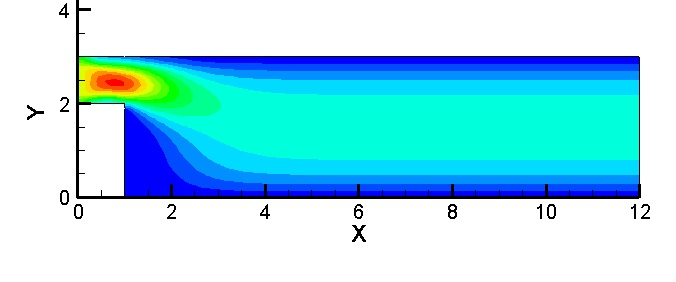
\includegraphics[width=150mm]{u1.jpg} \\
    


  \end{tabular}
\label{figur}\caption{Velocity contour for $Re=100$}
\end{figure}




\begin{figure}[htb]
  \centering
  \begin{tabular}{c}

    % Requires \usepackage{graphicx}

    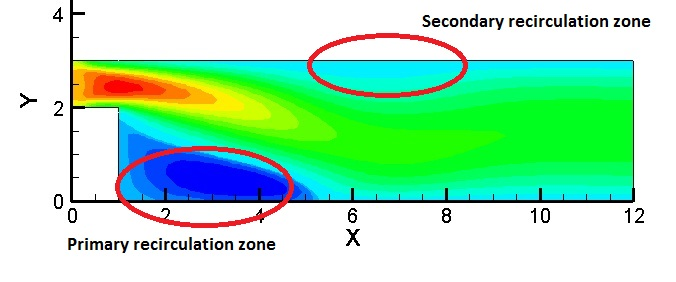
\includegraphics[width=150mm]{u5.jpg} \\

  \end{tabular}
\label{figur}\caption{Velocity contour for $Re=400$}
\end{figure}




\subsection{Residual}
One way to test the accuracy of CFD code is to validate physical laws or equations in the code. In order to do this for Incompressible Navier-Stokes equation, stream function   could be tracked in every iteration. If the difference of stream function values in $n$ and $n+1$ iteration decreases, it could be concluded that, the code is going to converge. It leads us to conservation of mass. \\
In Fig. (4), the residual for both stream function and vorticity are shown. It can be concluded that, steady state solution is occurred after 600 number of iteration. The accuracy of solution is in order of $10^{-4}$.

\begin{figure}[htb]
  \centering
  \begin{tabular}{c}

    % Requires \usepackage{graphicx}

    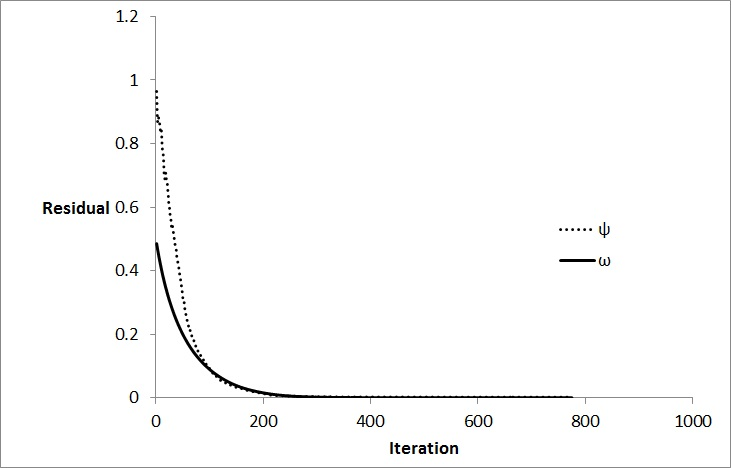
\includegraphics[width=150mm]{res.jpg} 


  \end{tabular}
\label{figur}\caption{Residual for stream function and vorticity}
\end{figure}


\begin{figure}[htb]
  \centering
  \begin{tabular}{c}

    % Requires \usepackage{graphicx}

    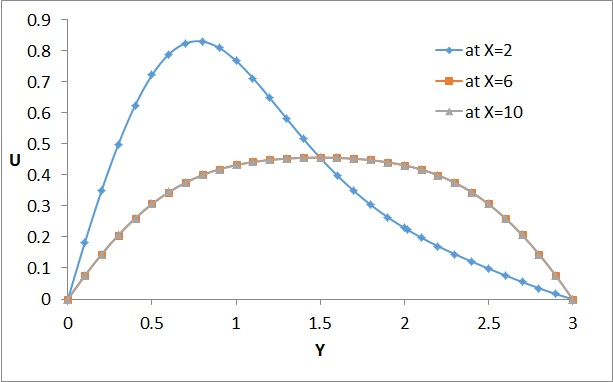
\includegraphics[width=100mm]{u1-1.jpg}    


  \end{tabular}
\label{figur}\caption{Velocity magnitude for different location in y direction, for  $Re=100.$}
\end{figure}

\begin{figure}[htb]
  \centering
  \begin{tabular}{c}

    % Requires \usepackage{graphicx}

    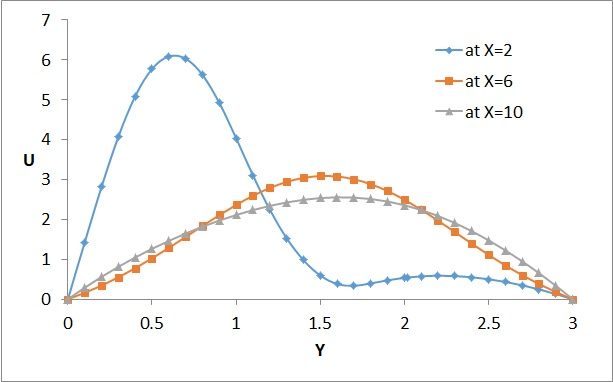
\includegraphics[width=100mm]{u2-1.jpg}
  \end{tabular}
\label{figur}\caption{Velocity magnitude for different location in y direction, from top to bottom $Re=200 .$}
\end{figure}


In Figs. (5-7), the velocity magnitude for different location in mesh domain is considered. They show that at first $(X=2)$ in the primary circulation zone, the velocity profile has slight change in magnitude but as $y$ increases, the profile going to be parabolic. This pattern is also illustrated for  $(X=6 \ and \ X=10)$ with smaller effect of step on velocity profile. This behavior increases as Reynolds number grows.

\begin{figure}[htb]
  \centering
  \begin{tabular}{c}

    % Requires \usepackage{graphicx}

    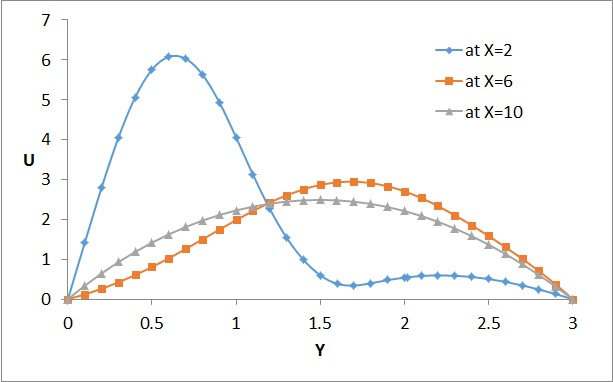
\includegraphics[width=100mm]{u5-1.jpg}    


  \end{tabular}
\label{figur}\caption{Velocity magnitude for different location in y direction, for $Re=400.$}
\end{figure}



\subsection{Scalibility}
As itwas mentioned before, to illustrate scalability, parallel programming on shared memory is used. Four different mesh sizes and three different computational procedure picked. In each mesh size, the running time of the code on machine calculated. As the number of CPUs increases, the running time would decrease. In Table (I), the running time is shown serial and parallel and in the Fig. (8) they are compared to ideal scalability.

\begin{figure}[htb]
  \centering
  \begin{tabular}{c}

    % Requires \usepackage{graphicx}

    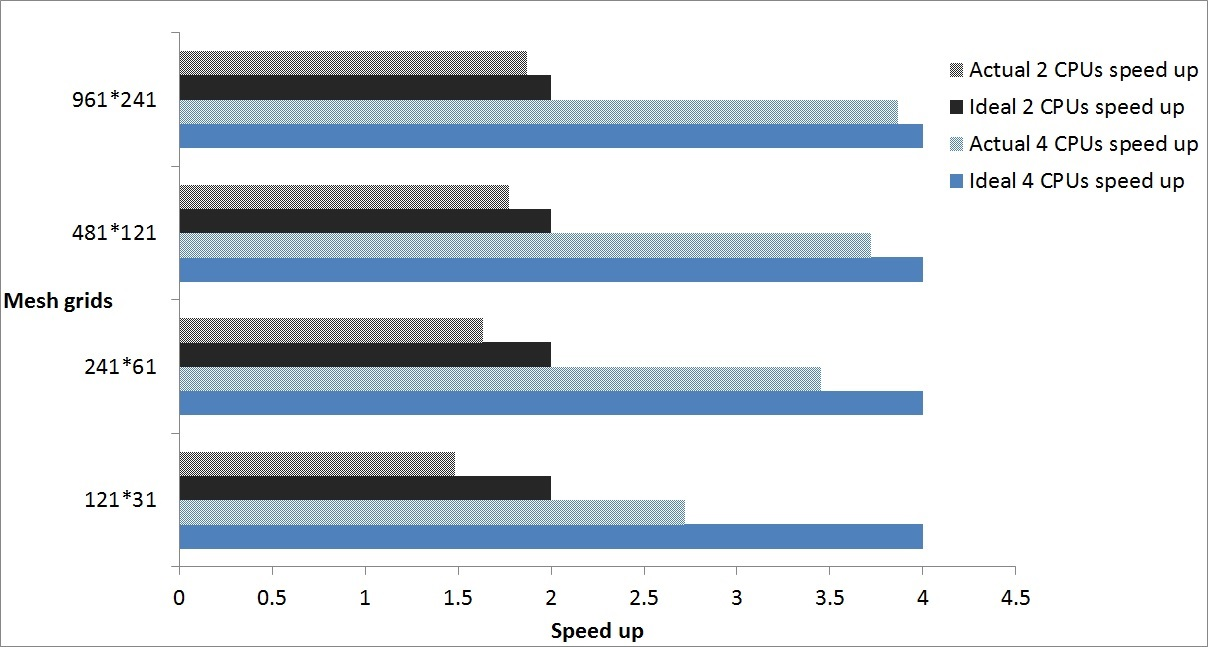
\includegraphics[width=150mm]{scale.jpg} 


  \end{tabular}
\label{figur}\caption{Speed up for different mesh grids and number of CPUs.}
\end{figure}


\begin{table}[htb]
\tbl{Run time for various grids and different number of CPUs in millisecond’s}{%
\begin{tabular}{|p{5pc}|p{5pc}|p{5pc}|p{5pc}|}
\hline

Mesh grids       & One CPU & Two CPUs & Four CPUs             \\[5pt] \hline
121*31        & 3622 	& 2436 & 1332	           \\ [5pt] \hline
241*61   & 30976          &  18948	    & 8965  \\ [5pt]  \hline
481*121   & 250352          &  141056	    & 67213  \\ [5pt]  \hline
961*241   & 2009519          &  1074875	    & 519814  \\  \hline  \\

\end{tabular}}

\label{tab1}
\end{table}


The number of mesh grids impact the run time of simulation. As it gets higher the speed up for two and four CPUs goes to two and four respectively. This scaling called weak speed up which is defined as how the solution time varies with the load per each CPU. 




\section{Conclusion}
The major numerical results are as follows. Contour plots of stream function, vorticity and velocities were presented at different Reynolds number. \\
I have presented accurate numerical solutions of the 2-D steady incompressible backward-facing step flow obtained using the upwind method. My results also indicate that the size of the recirculating regions grows  as the Reynolds number increases.

\section*{References}
1- Hoffmann, Klaus A., and Steve T. Chiang. "{Computational fluid dynamics, Vol. 1}." Wichita, KS: Engineering Education System (2000). \\
2-  Erturk, Ercan. "{Numerical solutions of 2-D steady incompressible flow over a backwardfacing step, Part I: High Reynolds number solutions}." Computers and Fluids 37.6 (2008) 633-655. \\

\section{Appendix}
\begin{lstlisting}[language=fortran]
! main program
program incompns
implicit none
integer,parameter :: imax=100
integer,parameter :: jmax=300

integer im,jm,k,i,j
real*8 psi(imax,jmax)
real*8 w(imax,jmax)
real*8 u(imax,jmax),v(imax,jmax)
real*8 check(imax,jmax)
real*8 dx,dy,duv
real*8 dt
real*8 nu
real*8 l,h
real*8 congs,conss
integer kmax
integer :: t1, t2,cr           ! timing variables

im=61
jm=61

l=12.0
h=3.0
dx=l/dfloat(im-1)
dy=h/dfloat(jm-1)
dt=0.001
nu=0.0025
congs=0.001
conss=0.002

! use only two threads
  !$ call omp_set_num_threads(4)
  
call system_clock( t1,cr )


do i=1,im
	do j=1,jm
		check(i,j)=0.0
	enddo
enddo

do i=1,10
	do j=1,10
		check(i,j)=1.0
	enddo
enddo


kmax=100
k=0
!!!!!!!!!!!!!!!!!!!!!!!!!!!!!!!!!!!!!!!
! variable intialization
call initial(im,jm,psi,w,u,v)

5	continue

k=k+1

call boundary_condition(im,jm,dx,dy,psi,w,u,v)

call update_omega(im,jm, dx, dy, w, u, v)


call ftcs(im,jm, dx, dy,dt, w, u, v, nu)

call pgs(im,jm, dx, dy, psi, w, congs)

call boundary_condition(im,jm,dx,dy,psi,w,u,v)

call velocity(im,jm, dx, dy, psi, u, v, duv)


call system_clock( t2,cr )
	
!!!!!!!!!!!!!!!!!!!!!!!!!!!!!!!!!!!!!!!
!display variation of velocity 

write(*,15) k, duv
15	format(2x, 'at iteration', i6, ', duv= ', f10.5)
!!!!!!!!!!!!!!!!!!!!!!!!!!!!!!!!!!!!!!!
! checking convergence

if(k.gt.kmax) then
	write(*,10) kmax
10	format (2x, 'no convegence reached in', i6, 'iteration')
else if (duv.gt.conss) then
	goto 5
	
endif

write(*,*) 'cpu_time in ms=', (t2-t1)*1000/cr
!!!!!!!!!!!!!!!!!!!!!!!!!!!!!!!!!!!!!!!!
! write reasult in files

call write_in_file(im,jm, dx, dy, psi, w, u, v)

end program incompns
!!!!!!!!!!!!!!!!!!!!!!!!!!!!!!!!!!!!!!!!
! initial subroutine

subroutine initial(im,jm, psi, w, u, v)
implicit none
integer,parameter :: imax=100
integer,parameter :: jmax=300

integer im,jm,k, i, j
real*8 psi(imax,jmax)
real*8 w(imax,jmax)
real*8 u(imax,jmax),v(imax,jmax)
real*8 dx,dy
real*8 dt
real*8 nu
real*8 l,h
real*8 congs,conss
integer kmax

	!$omp parallel default(none) &
    !$omp private(i,j)
     
    !$omp do

do i=1,im
	do j=1, jm
	
		psi(i,j)= 0.0
		w(i,j)= 0.0
		u(i,j)= 0.0
		v(i,j)= 0.0
	enddo
enddo

	!$omp end do
    !$omp end parallel
	
return
end subroutine initial
!!!!!!!!!!!!!!!!!!!!!!!!!!!!!!!!!!!!!!!!
! boundary condition subroutine

subroutine boundary_condition(im, jm, dx, dy, psi, w, u, v)
implicit none
integer,parameter :: imax=100
integer,parameter :: jmax=300

integer im,jm,k, i, j
real*8 psi(imax,jmax)
real*8 w(imax,jmax)
real*8 u(imax,jmax),v(imax,jmax)
real*8 dx,dy
real*8 dt
real*8 nu
real*8 l,h
real*8 congs,conss
integer kmax
real*8 :: psi_0, psi_20, psi_25, psi_30
integer i1,i2, i3, i4, j1, j2, j3
real*8 dx2, dy2

dx2=dx*dx
dy2=dy*dy

i1=20
j1=20
j2=6
j3=21

psi_0=0.0
psi_20=20.0
psi_25=25.0
psi_30=10.0

!!!!!!!!!!!!!!!!!!!!!!!!!!!!!!!!!!!!!!!
! boundary condition for psi

do i=1, i1
	psi(i,j1)= psi_0
enddo

do j=1, j1
	psi(i1,j)= psi_0
enddo

do i=i1+1, im
	psi(i,1)= psi_0
enddo

do i=1,im
	psi(i, jm)=psi_30
enddo

do j=j1+1,jm
	psi(1,j)= psi(2,j)
enddo


do j=1,jm
	psi(im, j)= psi(im-1,j)
enddo

!!!!!!!!!!!!!!!!!!!!!!!!!!!!!!!!!!!
! boundary condition for vorticity w
do i=1,i1
	w(i,j1)= 2.0*(psi(i,j1)-psi(i,j1+1))/dy2
enddo

do j=1,j1
	w(1,j)= 2.0*(psi(i1,j)-psi(i1+1,j))/dx2
enddo

do i=i1+1,im
	w(i,j1)= 2.0*(psi(i,1)-psi(i,2))/dy2
enddo



do i=1,im
	w(i, jm)= -2.0*(psi(i,jm)-psi(i,jm-1))/dy2
enddo


do j=j1,jm-1
	w(1,j)= 2.0*(psi(1,j)-psi(2,j))/dx2 &
		-(psi(1,j+1)-2.0*psi(1,j)+psi(1,j-1))*dy2
enddo


do j=1,jm
	w(im, j)= 2.0*(psi(im,j)-psi(im-1,j))/dx2 &
		-(psi(im,j+1)-2.0*psi(im,j)+psi(im,j-1))*dy2
enddo
!!!!!!!!!!!!!!!!!!!!!!!!!!!!!!!!!!!!!!!!!
! boundary condition for velocity 

do i=i1+1,im-1
		u(i,1)=0.0
		v(i,1)=0.0
enddo

do i=1,i1
		u(i,j1+1)=0.0
		v(i,j1+1)=0.0
enddo

do j=1,j1
		u(i1,j)=0.0
		v(i1,j)=0.0
enddo


!!!!!!!!!!!!!!!!!!!!!!!!!!!
do i=1,im
		u(i,jm)=0.0
		v(i,jm)=0.0
enddo


do j=j1,jm-1
		u(i,1)=-(psi(1,j1+1)-psi(1,j1))/dx
		v(i,1)=0.0
enddo



do j=1,jm-1
		u(i,1)=-(psi(im,j+1)-psi(im,j))/dx
		v(i,1)=0.0
enddo

u(im,jm)=0.0
v(im,jm)=0.0

return

end subroutine boundary_condition
!!!!!!!!!!!!!!!!!!!!!!!!!!!!!!!!!!!!!!!!
! subroutine update_omega

subroutine update_omega(im,jm,dx,dy,w,u,v)
implicit none
integer,parameter :: imax=100
integer,parameter :: jmax=300

integer im,jm,k, i, j,i1,j1
real*8 psi(imax,jmax)
real*8 w(imax,jmax)
real*8 u(imax,jmax),v(imax,jmax)
real*8 check(imax,jmax)
real*8 dx,dy
real*8 dt
real*8 nu
real*8 l,h
real*8 congs,conss
integer kmax
real*8 dvdx, dudy

i1=20
j1=20	
	
	!$omp parallel default(none) &
    !$omp private(i,j)
     
    !$omp do
	
do i=2,im-1
	j=0
	if(i<i1) j=j1
	do j=2,jm-1
		dvdx=(v(i+1,j)-v(i-1,j))/2.0/dx
		dudy=(u(i,j+1)-u(i,j-1))/2.0/dy
		w(i,j)= dvdx-dudy
	enddo
enddo

	!$omp end do
	!$omp end parallel
	
return
end subroutine update_omega
!!!!!!!!!!!!!!!!!!!!!!!!!!!!!!!!!!!!!!!!
! subroutine ftcs for vorticity unsteady equation

subroutine ftcs(im,jm,dy,dt,w,u,v,nu)
implicit none
integer,parameter :: imax=100
integer,parameter :: jmax=300

integer im,jm,k, i, j,i1,j1
real*8 psi(imax,jmax)
real*8 w(imax,jmax)
real*8 u(imax,jmax),v(imax,jmax)
real*8 check(imax,jmax)
real*8 dx,dy
real*8 dt
real*8 nu
real*8 l,h
real*8 congs,conss
integer kmax
real*8 dw(imax,jmax)
real*8 dx2,dy2,dx22,dy22
real*8 udwdx, vdwdy, d2wdx2, d2wdy2

dx2=dx*dx
dy2=dy*dy
dx22=2.0*dx
dy22=2.0*dy

i1=20
j1=20
	!$omp parallel default(none) &
    !$omp private(i,j)
     
    !$omp do
do i=2,im-1
	j=0
	if(i<i1) j=j1
	do j=2,jm-1
		udwdx= u(i,j)*(w(i+1,j)-w(i-1,j))/dx22
		vdwdy= v(i,j)*(w(i,j+1)-w(i,j-1))/dy22
		
		d2wdx2= (w(i+1,j)-2.0*w(i,j)+w(i-1,j))/dx2
		d2wdy2= (w(i,j+1)-2.0*w(i,j)+w(i,j-1))/dy2
		
		dw(i,j)=dt*(-(udwdx+vdwdy)+nu*(d2wdx2+d2wdy2))
	enddo
enddo

	!$omp end do
	!$omp end parallel
	
	
	!$omp parallel default(none) &
    !$omp private(i,j)
     
    !$omp do
do i=2,im-1
	j=0
	if(i<i1) j=j1
	do j=2,jm-1
		w(i,j)= w(i,j)+dw(i,j)
	enddo
enddo

	!$omp end do
	!$omp end parallel
return
end subroutine ftcs
!!!!!!!!!!!!!!!!!!!!!!!!!!!!!!!!!!!!!!!!!!
! subroutine point gauss-seidel

subroutine pgs(im,jm,dx,dy,psi,w,congs)
implicit none
integer,parameter :: imax=100
integer,parameter :: jmax=300

integer im,jm,k, i, j,i1,j1
real*8 psi(imax,jmax)
real*8 w(imax,jmax)
real*8 u(imax,jmax),v(imax,jmax)
real*8 check(imax,jmax)
real*8 dx,dy
real*8 dt
real*8 nu
real*8 l,h
real*8 congs,conss
integer kmax
real*8 psi_old,error,errinit,err

real*8 :: dx2,dy2,beta2,cxy

dx2=dx*dx
dy2=dy*dy
beta2=(dx2/dy2)
cxy=0.5/(1.0+beta2)
k=0

i1=20
j1=20

5 continue 

k=k+1
error=0.0
	
	!$omp parallel default(none) &
    !$omp private(i,j)
     
    !$omp do

do i=2,im-1
	j=0
	if(i<i1) j=j1
	do j=2,jm-1
		psi_old=psi(i,j)
		psi(i,j)=cxy*(dx2*w(i,j)+psi(i+1,j)+psi(i-1,j) &
			+beta2*(psi(i,j+1)+psi(i,j-1)))
		error=error+abs(psi(i,j)-psi_old)
		
		if(k.eq.1) then
		errinit=error
		endif
	enddo
enddo
	!$omp end do
	!$omp end parallel
	
err=error/errinit

if(k.gt.10000) then 
	write(*,100) 
else
	if(err.gt.congs) then
	goto 5
	endif
endif

100 format (2x, 'pgs did not converge in 10000 iterations')

return

end subroutine pgs
!!!!!!!!!!!!!!!!!!!!!!!!!!!!!!!!!!!!!!!!!!!!!!!
! subroutine velocity

subroutine velocity(im,jm,dx,dy,psi,u,v,duv)
implicit none
integer,parameter :: imax=100
integer,parameter :: jmax=300

integer :: im,jm,k, i, j,i1,j1
real*8 psi(imax,jmax)
real*8 w(imax,jmax)
real*8 u(imax,jmax),v(imax,jmax)
real*8 check(imax,jmax)
real*8 dx,dy,duv
real*8 dt
real*8 nu
real*8 l,h
real*8 congs,conss
integer kmax
real*8 	 unew,vnew
real*8 	 num,denum

num=0.0
denum=0.0
i1=20
j1=20
	!$omp parallel default(none) &
    !$omp private(i,j)
     
    !$omp do
do i=2,im-1
	j=0
	if(i<i1) j=j1
	do j=2,jm-1
		unew= (psi(i,j+1)-psi(i,j-1))/2.0/dy
		vnew= (psi(i+1,j)-psi(i-1,j))/2.0/dx
		num=num+ sqrt((unew-u(1,j))**2.0+ (vnew-v(i,j))**2.0)
		u(i,j)=unew
		v(i,j)=vnew
	enddo
enddo
	!$omp end do
	!$omp end parallel
	
	!$omp parallel default(none) &
    !$omp private(i,j)
     
    !$omp do
do i=2,im-1
	j=0
	if(i<i1) j=j1
	do j=2,jm-1
		denum=denum+ sqrt(u(i,j)**2.0+v(i,j)**2.0)
	enddo
enddo
	!$omp end do
	!$omp end parallel
duv=num/denum
return

end subroutine velocity
!!!!!!!!!!!!!!!!!!!!!!!!!!!!!!!!!!!!!!!!!!
! subroutine write_in_file
subroutine write_in_file(im,jm,dx,dy,psi,w,u,v)
implicit none
integer,parameter :: imax=100
integer,parameter :: jmax=300

integer im,jm,k, i, j
real*8 psi(imax,jmax)
real*8 w(imax,jmax)
real*8 u(imax,jmax),v(imax,jmax)
real*8 check(imax,jmax)
real*8 dx,dy
real*8 dt
real*8 nu
real*8 l,h
real*8 congs,conss
integer kmax
open(1,file='pbs8.dat')
write(1,111)im,jm,dx,dy
111 format ('im=', i4, ' ; jm=',  i4, '; dx=', f5.3, ';dy=', f5.3)

!!!!!!!!!!!!!!!!!!!!!!!!!!!!!!!!!!!!!!!!!!
write(1,*) 'stream function distribuation'
write(1,*) 
write(1,100) ((i-1)*dx, i=1,im,5)

do j=jm,1,-1
	write(1,200) (j-1)*dy, (psi(i,j), i=1,im,5)
enddo

write(1,*)
write(1,*)
write(1,*)
!!!!!!!!!!!!!!!!!!!!!!!!!!!!!!!!!!!!!!!!!!
write(1,*) 'vorticity distribution'
write(1,*)
write(1,100) ((i-1)*dx, i=1,im,5)

do j=jm,1,-1
	write(1,200) (j-1)*dy, (w(i,j), i=1,im,5)
enddo

write(1,*)
write(1,*)
write(1,*)
!!!!!!!!!!!!!!!!!!!!!!!!!!!!!!!!!!!!!!!!!!!
write(1,*) 'u component of velocity'
write(1,*)
write(1,100) ((i-1)*dx, i=1,im,5)

do j=jm,1,-1
	write(1,200) (j-1)*dy, (u(i,j), i=1,im,5)
enddo

write(1,*)
write(1,*)
write(1,*)
!!!!!!!!!!!!!!!!!!!!!!!!!!!!!!!!!!!!!!!!!!!
write(1,*) 'v component of velocity'
write(1,*)
write(1,100) ((i-1)*dx, i=1,im,5)

do j=jm,1,-1
	write(1,200) (j-1)*dy, (v(i,j), i=1,im,5)
enddo

write(1,*)
write(1,*)
write(1,*)
!!!!!!!!!!!!!!!!!!!!!!!!!!!!!!!!!!!!!!!!!!!

100 format(14x, 'y', 11('x=', f3.1, 6x))
200 format(f17.3, 2x, 11('x=', f3.1, 6x))
close(1)
!!!!!!!!!!!!!!!!!!!!!!!!!!!!!!!!!!!!!!!!!!!
open(2, file='pbs8.dat')
write(2,221)
write(2,222)
write(2,223) im, jm
221 format(1x, 'title="psi,w,u,v,velocity"')
222 format(1x, 'variables= "x", "y", "psi", "w", "u", "v","velocity" ')
223 format(1x, 'zone t= "l", i=', i3, 2x, 'j=', i3,2x, 'f=point')

do  j=1,jm
	do i=1,im
		write(2,224) (i-1)*dx, (j-1)*dy, psi(i,j), w(i,j), u(i,j), v(i,j), sqrt(u(i,j)**2+v(i,j)**2)
	enddo
enddo

224 format (7(2x,d14.8))
close(2)

return

end subroutine write_in_file
!!!!!!!!!!!!!!!!!!!!!!!!!!!!!!!!!!!!!!!!!!!!
\end{lstlisting}

\end{document}
% End of v2-acmlarge-sample.tex (March 2012) - Gerry Murray, ACM




